\chapter{Model framework}
\label{chapter:BackgroundLit}
\begin{lstlisting}[language=Python]
# Monte Carlo spreidingsdiagram: belasting M_E tegen sterkte M_R
C_SAFE, C_FAIL, INK, MUTED = "#2a78d6", "#d03b3b", "#9b9b9b", "#52514e"
n_plot = 5_000                                    # subset voor leesbaarheid
idx = rng.choice(N, n_plot, replace=False)
Z = M_R - M_E                                     # veiligheidsmarge [kNm/m]

fig, (ax1, ax2) = plt.subplots(1, 2, figsize=(12, 5))

ok = ~faalt[idx]
ax1.scatter(M_E[idx][ok], M_R[idx][ok], s=8, c=C_SAFE, alpha=0.35, lw=0,
            label="Veilig (M_R >= M_E)")
ax1.scatter(M_E[idx][~ok], M_R[idx][~ok], s=8, c=C_FAIL, alpha=0.35, lw=0,
            label="Faalt (M_R < M_E)")
lim = max(np.percentile(M_E, 99.9), np.percentile(M_R, 99.9))
ax1.plot([0, lim], [0, lim], c=INK, lw=1.5, ls="--", label="Grenstoestand M_R = M_E")
ax1.set_xlim(0, lim); ax1.set_ylim(0, lim); ax1.set_aspect("equal")
ax1.set_xlabel("Belasting M_E [kNm/m]"); ax1.set_ylabel("Sterkte M_R [kNm/m]")
ax1.set_title(f"Monte Carlo spreiding ({n_plot:,} van {N:,} trekkingen)", loc="left")
ax1.legend(frameon=False, loc="upper left")

bins = np.linspace(np.percentile(Z, 0.1), np.percentile(Z, 99.9), 80)
ax2.hist(Z[Z >= 0], bins=bins, color=C_SAFE, alpha=0.8, label="Veilig")
ax2.hist(Z[Z < 0], bins=bins, color=C_FAIL, alpha=0.8, label="Faalt")
ax2.axvline(0, c=INK, lw=1.5, ls="--")
ax2.set_xlabel("Veiligheidsmarge Z = M_R - M_E [kNm/m]")
ax2.set_ylabel("Aantal trekkingen")
ax2.set_title(f"Faalkans P(Z < 0) = {faalt.mean():.3f}", loc="left")
ax2.legend(frameon=False)

for ax in (ax1, ax2):
    ax.spines[["top", "right"]].set_visible(False)
    ax.grid(alpha=0.2, lw=0.5)
    ax.tick_params(colors=MUTED)

fig.tight_layout()
fig.savefig(FIGURES / "monte_carlo_spreiding.png", dpi=200, bbox_inches="tight")
plt.show()
\end{lstlisting}

Uncertain inputs, such as construction year, lifetime parameters and consequence weights, are described by probability distributions. Monte Carlo simulation samples these inputs and recalculates the ranking in each run. The spread of the results gives the confidence of the ranking, for instance the share of runs in which a segment belongs to the highest-risk group.

Monte Carlo simulation shows how uncertain the result is, but not which input causes that uncertainty. A separate sensitivity analysis is therefore performed. A tornado analysis first screens out inputs with little influence. Variance-based (Sobol) indices are then calculated for the remaining inputs. Inputs with a large influence on the ranking indicate where additional inspection or data collection is most valuable.

\section{NEN8700}
For existing structures, a statutory minimum level of structural safety applies. NEN 8700 can be used to assess whether an existing structure meets this level and whether structural measures are required. 

NEN8700 §3.5(5) says a check at rejection level may be based directly on probabilistic methods.\footnote{Voor grondslagen voor probabilistische methoden, zie bijlage C van NEN-EN 1990}
\begin{enumerate}
    \item Define a limit state for each failure mechanism: $g=R-S$, where the wall fails when $g < 0 $
    \item Given the variables distributions instead of feed values: soil strength, water levels, traffic load, wall thickness after corrosion or decay
    \item Calculate the failure probability with Monte Carlo or FORM, then \(\beta = -\phi^{-1}(P_f) \)
    \item Add evidence as conditional events: survival so far, or observed cracks and settlement
\end{enumerate}


\section{Monte Carlo example}

Drawing from Hemel et al. (2024), this is as a Monte Carlo example meant to demonstrate how a potential model operates. In the subsequent sections in this chapter, the models are therefore based on timber piles as outlined in the paper as a baseline for maintenance programming along Utrecht walls following data collection and variable definition.


\begin{lstlisting}[language=Python]
import numpy as np
rng = np.random.default_rng(1)
N = 100_000

# invoer: vast of verdeling
bouwjaar = rng.uniform(1960, 1980, N)
leeftijd = 2026 - bouwjaar
H   = rng.normal(1.5, 0.2, N)                      # kerende hoogte [m]
phi = rng.normal(30, 2, N)                         # hoek inwendige wrijving [graden]
gam = rng.normal(18, 1, N)                         # volumegewicht grond [kN/m3]
q   = rng.normal(5, 1.5, N).clip(0)                # verkeersbelasting [kN/m2]
t0  = rng.normal(0.060, 0.005, N)                  # oorspronkelijke dikte [m]
r   = rng.uniform(0, 0.001, N)                     # afname dikte [m/jaar]
fm  = rng.lognormal(np.log(18_000), 0.2, N)        # buigsterkte [kN/m2]

# formule
Ka = np.tan(np.radians(45 - phi / 2)) ** 2
M_E = Ka * gam * H**3 / 6 + Ka * q * H**2 / 2      # belasting [kNm/m]
t   = (t0 - r * leeftijd).clip(0.001)
M_R = fm * t**2 / 6                                # sterkte [kNm/m]

# resultaat
faalt = M_R < M_E
print("Faalkans:", faalt.mean())
\end{lstlisting}

\begin{figure}[ht]
    \centering
    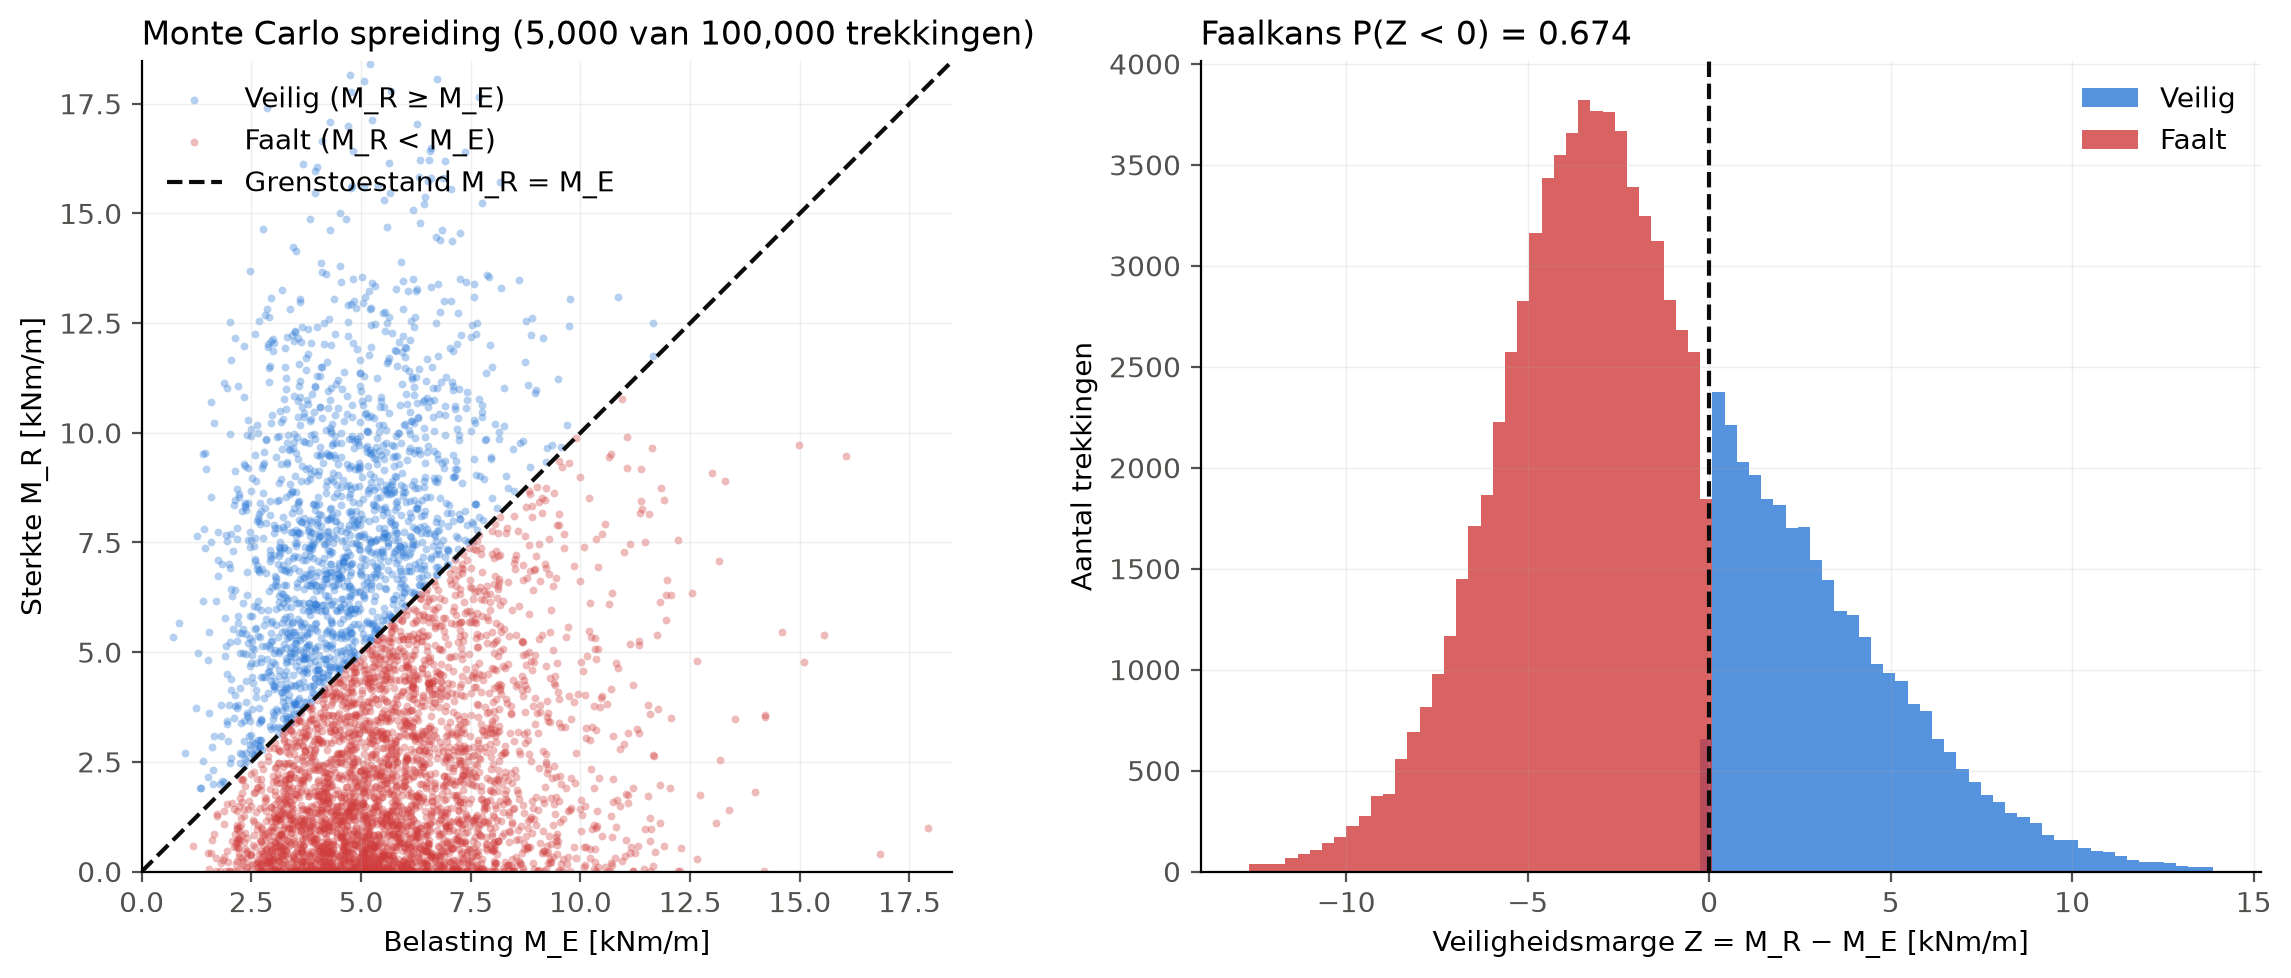
\includegraphics[width=0.75\linewidth]{figures/monte_carlo_spreiding.png}
    \caption{Example}
    \label{fig:placeholder}
\end{figure}



\section{Failure mechanism}
Lateral failure of the timber pile foundation. Earth pressure and traffic load push the wall towards the water and the piles bend. Failure is defined as the onset of yielding in the timber (Hemel et al., 2024).

\section{Limit state}
From Hemel et al. (2024), Eq.~3--4:
\begin{equation}
g(X,t) = MOR - \sigma_b(t), \qquad P_f = P\left[g(X,t) < 0\right]
\end{equation}
\begin{equation}
\sigma_b = \theta_M \frac{32\,M}{\pi D^3} + \theta_N \frac{4\,N}{\pi D^2}
\end{equation}

\section{Simplified bending stress (own calibration)}
We do not have the analytical pile model used by Hemel, so $M$ is replaced by a simple expression calibrated to the published case ($\beta \approx 1.5$ at $q = 7$ kN/m$^2$ over 15 years):
\begin{equation}
\sigma_b(t) = \theta_M\,\theta_S\,(s_0 + s_q\,q)\left(\frac{D_{ref}}{D(t)}\right)^4 + \theta_N \frac{4N}{\pi D(t)^2}
\end{equation}
\begin{equation}
D(t) = D_0 - r\,t
\end{equation}
with $s_0 = 3.0$ N/mm$^2$, $s_q = 0.10$ (N/mm$^2$)/(kN/m$^2$) and $D_{ref} = 240$ mm. The exponent 4 is a fitted value: $D$ acts on the stress through $D^3$ and on pile stiffness through $D^4$. The resulting influence factors (diameter 0.63, soil 0.14, load 0.07) are close to those in the paper (0.67, about 0.21, 0.07).

\section{Inputs}
\begin{tabular}{llll}
\toprule
Symbol & Meaning & Distribution & Source \\
\midrule
$D_0$ & Pile diameter now & Normal(245 mm, CoV 0.10) & Hemel 2024 \\
$r$ & Diameter loss by bacterial decay & 0.34 mm/yr & Hemel 2024 \\
$t$ & Time window & 15 yr & NEN 8700 \\
$MOR$ & Bending strength timber & Normal(22 N/mm$^2$, 0.10) & Hemel 2024 \\
$q$ & Traffic load & Normal(7 kN/m$^2$, 0.20) & Hemel 2024 \\
$\theta_M$ & Model uncertainty bending & Lognormal(1, 0.10) & JCSS \\
$\theta_N$ & Model uncertainty axial & Lognormal(1, 0.05) & JCSS \\
$\theta_S$ & Lumped soil uncertainty & Lognormal(1, 0.20) & Own calibration \\
$N$ & Axial force per pile & 20 kN & Own estimate \\
\bottomrule
\end{tabular}

Notes:
\begin{itemize}
  \item Replace Amsterdam values with Utrecht data where available (axle-load limits for $q$, diameter or soft-shell measurements for $D_0$ and $r$).
  \item The thesis (Hemel, 2023) finds a soft shell of 21 mm on average (max.\ 45 mm) and a CoV of 0.26 for MOR. Useful as a sensitivity case.
\end{itemize}

\section{Solving and assessment}
Crude Monte Carlo with $n \geq 10^5$:
\begin{equation}
P_f = \frac{1}{n}\sum_{j=1}^{n} \mathbf{1}\left[g(X_j,t) < 0\right], \qquad \beta = -\Phi^{-1}(P_f)
\end{equation}

Minimum reliability for existing structures, 15-year reference period (NEN 8700, Table B.2):

\begin{tabular}{lll}
\toprule
Consequence class & $\beta_{min}$ & $P_{f,max}$ \\
\midrule
CC1 & 1.8 & $3.6\cdot10^{-2}$ \\
CC2 & 2.5 & $6.2\cdot10^{-3}$ \\
CC3 & 3.3 & $4.8\cdot10^{-4}$ \\
\bottomrule
\end{tabular}

$P_f$ is the $P$ in the risk score $R = P \cdot C$ per structure.

\section{Optional: updating with past performance}
If a load $q_\eta$ is known to have been survived, evaluate the limit state a second time with $q_\eta$ and today's diameter, and keep only the surviving samples (Hemel et al., 2024, Eq.~12):
\begin{equation}
P_{f|\eta} = \frac{\sum_j \mathbf{1}\left[g(X_j,q_j)<0\right]\cdot \mathbf{1}\left[g(X_{\eta,j},q_{\eta,j})>0\right]}{\sum_j \mathbf{1}\left[g(X_{\eta,j},q_{\eta,j})>0\right]}
\end{equation}
In the paper, survival of 10 kN/m$^2$ raises $\beta$ from 1.5 to 2.0. Adding a measured displacement below 4 mm raises it to 3.2.

\section{Limitations}
\begin{itemize}
  \item Valid only for masonry walls on timber piles. Concrete revetments and sheet piling need other mechanisms (e.g.\ corrosion).
  \item Calibrated on one Amsterdam case. Suitable for relative comparison between structures, not for absolute failure probabilities.
  \item Inputs are treated as uncorrelated, which overestimates reliability. MOR and stiffness have a measured correlation of 0.83.
\end{itemize}